\subsection{Hàng đợi tranh chấp và các primitive hoàn thành (RQ1)}\label{sec:contention}
Kết quả quá tải quy cho khoảng cách hai cấu trúc đồng bộ idiom bắt buộc, nhưng
sự quy kết đó được lập luận từ hình dạng đo toàn dịch vụ. Tiểu mục này
cô lập riêng các cấu trúc đó.

\ContentionProducers{} luồng producer đập vào một hàng đợi có giới hạn dung lượng $1\,024$ trong khi một
consumer duy nhất rút khỏi đó. Mỗi producer gửi một job không làm gì mang tay cầm hoàn thành một lần và chặn
cho đến khi consumer báo hiệu. Không có công việc \texttt{ShardCore} nào chạy trên đường đi. C++ dùng
\texttt{BoundedQueue} viết tay của Mục~\ref{sec:impldetails} với
\texttt{std::promise}/\texttt{std::future}. Rust dùng \texttt{sync\_channel} và một
\texttt{mpsc::channel()} mới mỗi yêu cầu. Mỗi cửa sổ đo kéo dài hai giây sau khởi động nóng.
\ContentionRepeats{} lần lặp xen kẽ được tóm tắt bằng trung vị với khoảng bootstrap và
kiểm định bằng thủ tục hoán vị ghép cặp chính xác của Mục~\ref{sec:stats}.
Bảng~\ref{tab:contention} báo cáo kết quả.

\begin{table}[H]
\centering
\small
\caption[Thông lượng qua các primitive đồng bộ tranh chấp riêng]{Thông lượng qua
hàng đợi có giới hạn và các primitive hoàn thành riêng, với \ContentionProducers{} producer tranh chấp
và dung lượng hàng đợi $1\,024$. Giá trị là trung vị trên \ContentionRepeats{} lần lặp xen kẽ phía trên
khoảng tin cậy bootstrap $95\%$. Kiểm định ghép cặp so C++ với Rust trên thông lượng
bền vững (kops/s). Đo trên máy chủ của Mục~\ref{sec:testbed}.\label{tab:contention}}
\begin{tabular}{@{}l r r r@{}}
\hline\hline
Ngôn ngữ & Thông lượng (kops/s) & Trung bình ns/op & $p$ ghép cặp \\
\hline
C++ & \mci{55.0}{53.7}{58.4} & \mci{18178}{17110}{18632} & \multicolumn{1}{c}{---} \\
Rust & \mci{58.7}{56.8}{61.8} & \mci{17045}{16169}{17594} & 0.226
\\
\hline
\end{tabular}
\end{table}

Các primitive cô lập không tái tạo thứ tự quá tải. C++ duy trì
\ContentionThrCpp{}~kops/s và Rust \ContentionThrRust{}~kops/s, khoảng cách chỉ
$\ContentionRatio\times$ với $p = \ContentionP$. Toàn dịch vụ ở
$\OverloadLoad$~kops/s tách $\OverloadThrRatio\times$, với $p$ đã hiệu chỉnh ở
sàn của họ. Cách đọc trung thực do đó là sự phân kỳ quá tải gồm thêm
công việc mà microbenchmark loại bỏ: \texttt{Request} gắn thẻ lớn hơn phía C++, 
điều phối variant của worker, và các thao tác bản đồ vẫn chạy trong chế độ quá tải.
Điều kết quả vẫn thiết lập hữu ích. Khác biệt bậc độ lớn chỉ ở primitive
bị loại trừ, và tìm cơ chế chuyển sang phần còn lại của đường bàn giao chứ không
sang mô hình an toàn.

\subsection{Sử dụng tài nguyên (RQ3)}\label{sec:resources}
Bảng~\ref{tab:resource} báo cáo sử dụng tài nguyên ở cùng
tải bền vững. Peak resident set size tách bốn biến thể rõ ràng, và tách vậy
dù đọc họ theo cách nào. Khoảng của nó loại trừ không, và hiệu ứng giữ dấu dưới
cả hai bộ cấp phát. Hình~\ref{fig:resources} vẽ cùng phép đo. Panel giữa là
nơi phát hiện của mục này nằm, với hai hiệu ứng bên trong peak RSS vẽ thành
khác biệt ghép cặp trên một trục chung.

Hai hiệu ứng có trong đó, không phải một, và chúng không cùng cỡ. Liên kết
\texttt{jemalloc} tốn $\RssAllocDiffLo$--$\RssAllocDiffHi$~MiB ở cả hai ngôn ngữ. Bản build Rust
tốn thêm $\RssLangDiffLo$--$\RssLangDiffHi$~MiB so với bản build C++ dưới cả hai bộ cấp phát,
với khoảng bootstrap $\RssLangCILo$ đến $\RssLangCIHi$~MiB. Sử dụng tài nguyên theo cả hai, và
hiệu ứng bộ cấp phát lớn hơn một bậc độ lớn. Thứ tự đó phần nào đến từ
kiểm soát công bằng chứ không phải sự thật chung về \texttt{jemalloc}. Cả hai build ghim số arena
giống nhau, để mặc định của không ngôn ngữ nào thành lợi thế tình cờ, và
ghim cao là điều làm metadata arena thành chi phí cố định lớn hai bên. Triển khai
tinh chỉnh \texttt{jemalloc} cho dấu chân thay vì so sánh công bằng sẽ không trả chi phí đó.

Hàng duy nhất trong khối trên của Bảng~\ref{tab:significance} không vượt
hiệu chỉnh là peak RSS dưới
\texttt{jemalloc}, và lý do nằm ở thống kê chứ không phải phần mềm.
Khoảng ở đó chặt, xa không, và $18$ trong $20$ lần lặp ghép cặp đồng ý. Điều đánh bại kiểm định là vài lần chạy báo resident set thấp hơn trung vị biến thể khoảng $30$~MiB
trong khi vẫn không phân biệt được về thông lượng, thời gian tường và số lỗi. Thống kê
hoán vị là trung bình khác biệt ghép cặp, và một lần chạy như vậy chi phối nó. Đây là trường hợp
quy tắc đọc của Mục~\ref{sec:stats} được viết trước để bao phủ, và
Mục~\ref{sec:threats} tiếp nhận cả quy tắc và khuyết điểm đo đằng sau nó.

Sử dụng CPU hành xử khác cả hai, và khác biệt phụ thuộc chế độ chứ không
phải nhiễu. Ở điểm vận hành dưới bão hoà này Rust tiêu thụ CPU \emph{ít} hơn một chút, tối đa
$\CpuDiffAbsMax$ điểm phần trăm, nhất quán dưới cả hai bộ cấp phát và vượt
hiệu chỉnh dưới cả hai. Mục~\ref{sec:overload} thấy dấu đảo qua bão hoà và
biên độ lớn hơn nhiều. Thông lượng đạt được không thêm gì ở đây, vì lý do
Mục~\ref{sec:stats} nêu. Ở điểm dưới bão hoà nó bị ghim vào tải đề nghị, và
chỉ báo cáo để xác nhận điểm được duy trì chứ không chỉ danh nghĩa, và nó vậy trong
$\ReprLoadShortfall\%$.

Hai điều kiện giữ phát hiện bộ nhớ đúng cỡ thực tế. Đó là khác biệt chi phí cố định
chứ không phải chi phí mỗi ngữ cảnh. Ở $5\,000$ UE hoạt động dùng trong quét,
khác biệt bố cục tám byte đo ở Mục~\ref{sec:uecontext} chiếm khoảng
$40$~kB, thiếu hai bậc độ lớn so với khoảng cách. Phần lớn khoảng cách do đó là overhead runtime và
arena bộ cấp phát, không tỷ lệ với khối lượng công việc và sẽ quan trọng tỷ lệ
ít hơn trong triển khai lớn hơn, không phải nhiều hơn. Điều kiện thứ hai là phép đo
thiết lập khác biệt mà không giải thích. Không thu bộ đếm phần cứng hay hồ sơ cấp phát,
nên phần chia giữa dự trữ arena, bộ nhớ đệm mỗi luồng và dấu chân tĩnh
không được giải quyết ở đây. Cả hai điểm được xem lại ở Chương~\ref{chapter:discussion}.

Phát hiện RQ3 do đó không phải ``không phạt tài nguyên'' phẳng mà khoảng chồng lấn
gợi ý, cũng không phải phạt hiệu năng chung. Rust tốn thêm vài megabyte dấu chân cố định, tái lập được và dưới cả hai bộ cấp phát, nhưng nhỏ hơn một bậc độ lớn so với chính lựa chọn
bộ cấp phát. Nó rẻ hơn một chút về CPU khi dịch vụ còn chịu tải, và đắt hơn đáng kể khi không còn.
Trên thao tác trần của Mục~\ref{sec:budget} nó là ngôn ngữ
nhanh hơn trong hai.

\begin{table}[H]
\centering
\small
\caption[Sử dụng tài nguyên ở tải đại diện]{Sử dụng tài nguyên ở tải đề nghị bền vững $\ReprLoad$~kops/s: thông lượng đạt được,
peak RSS và tổng sử dụng CPU. Trung vị trên \NRepeats{} lần lặp phía trên khoảng tin cậy bootstrap
$95\%$. Peak RSS là chỉ số duy nhất ở đây mà khoảng tách bốn
biến thể rõ ràng.\label{tab:resource}}
\begin{tabular}{@{}l r r r@{}}
\hline\hline
Biến thể & thông lượng (kops/s) & peak RSS (MiB) & CPU (\%) \\
\hline
C++ (system alloc) & \mci{27.99}{27.99}{27.99} & \mci{9.4}{9.4}{9.5} & \mci{66.8}{65.8}{68.2} \\
C++ (jemalloc) & \mci{27.95}{27.95}{27.96} & \mci{65.9}{65.9}{65.9} & \mci{64.6}{63.4}{66.1} \\
Rust (system alloc) & \mci{27.99}{27.99}{27.99} & \mci{11.2}{11.1}{11.3} & \mci{63.3}{62.2}{66.0} \\
Rust (jemalloc) & \mci{27.95}{27.92}{27.96} & \mci{67.2}{65.4}{67.3} & \mci{63.0}{62.4}{64.5}
\\
\hline
\end{tabular}
\end{table}

\begin{figure}[ht]
\centering
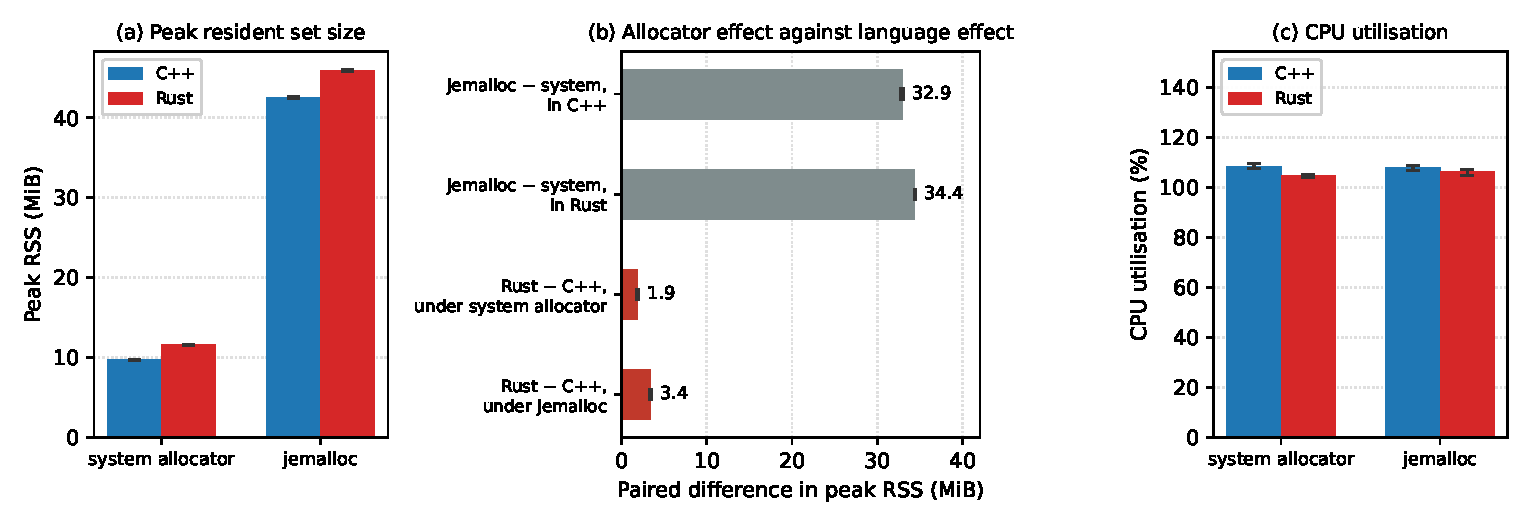
\includegraphics[width=0.78\linewidth]{figures/fig_resources.pdf}
\caption[Sử dụng tài nguyên và hai hiệu ứng trong peak RSS]{Sử dụng tài nguyên ở tải đề nghị bền vững $\ReprLoad$~kops/s, nhóm theo bộ cấp phát để
hai cột trong nhóm chỉ khác ngôn ngữ và hai nhóm chỉ khác bộ cấp phát.
Trung vị trên \NRepeats{} lần lặp với khoảng bootstrap $95\%$. \textbf{(a)} Kích thước resident set đỉnh.
\textbf{(b)} Hai hiệu ứng nó chứa, mỗi cái là khác biệt ghép cặp trên cùng
lần lặp: liên kết \texttt{jemalloc} tốn $\RssAllocDiffLo$--$\RssAllocDiffHi$~MiB, trong khi bản build Rust
tốn thêm $\RssLangDiffLo$--$\RssLangDiffHi$~MiB so với bản C++. Cả hai đều thật, và trên
trục chung hiệu ứng bộ cấp phát lớn hơn một bậc độ lớn. \textbf{(c)} Sử dụng
CPU, cộng qua các luồng, nơi khác biệt chạy chiều ngược và
nhỏ.\label{fig:resources}}
\end{figure}

